This tutorial draws on cylc and rose documentation:

\begin{itemize}
    \item \url{http://cylc.github.io/cylc}
    \item \url{http://metomi.github.io/rose}
\end{itemize}


\section{Cylc Overview}

Cylc (``silk'') is a workflow engine that can manage continuous workflows of
cycling (repeating) tasks for applications such as weather and environmental
forecasting, and climate simulation.  It employs a novel self-organising
scheduling algorithm that is simple but powerful: in an evolving task pool,
tasks (which know their own private inputs, outputs, and cycle point) can
submit their jobs to run once their inputs have been satisfied by the
completed outputs of other tasks.

A {\em task} is an abstract representation of a {\em job} that runs on a
computer, and a {\em workflow} is a {\em suite} of interdependent tasks.
Here's a small workflow of six tasks (with no cycling as yet):

\begin{center}
    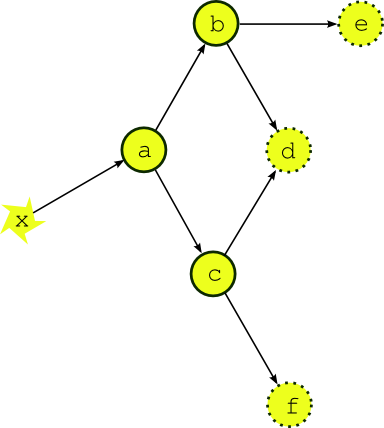
\includegraphics[width=0.25\columnwidth]{resources/tex/dep-one-cycle}
\end{center}

Graph {\em nodes} represent tasks, and {\em edges} (arrows) represent
dependence.  For instance, task {\em a} might write out data files that are
read in by tasks {\em b} and {\em c}.  The node {\em x} represents an external
event such as receipt of new real-time weather observations.  Here's the
optimal job schedule for this workflow,

\begin{center}
    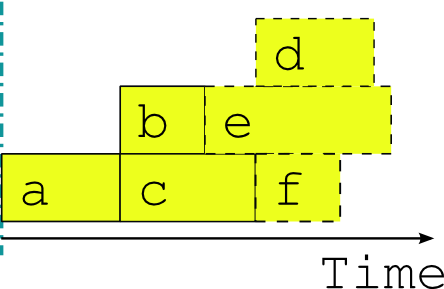
\includegraphics[width=0.2\columnwidth]{resources/tex/timeline-zero.png}
\end{center}

(Bar width is proportional to task run time, and the vertical axis is
meaningless). So {\em b} and {\em c} start running at the same time, immediately
after {\em a} finishes, and so on. Before running the workflow repeatedly ({\em
cycling} it) we should look out for {\em inter-cycle dependence}.   For
example, task {\em a} may depend on restart files generated by its own previous
instance, like this:

\begin{center}
    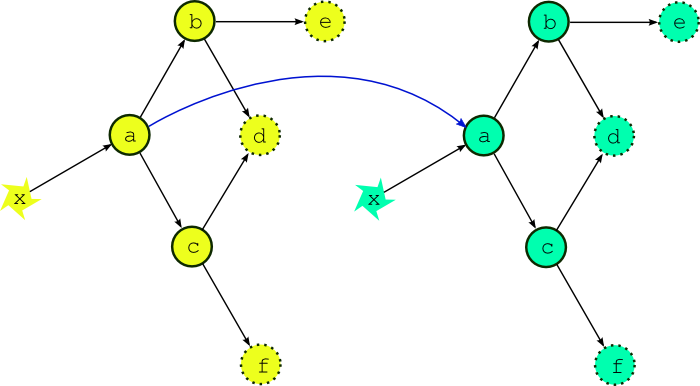
\includegraphics[width=0.5\columnwidth]{resources/tex/dep-two-cycles-linked}
\end{center}

In normal real time operation we can ignore the inter-cycle dependence because
one cycle always completes before the next can start (when the next external
data comes in).  But if the suite has to catch up from a long delay or outage,
or if we run it over archived historical data, it should be able to run tasks
from multiple cycles at once for more efficient scheduling: if the next {\em x}
is already done then the next {\em a} should be able to start as soon as the
current {\em a} has finished, even if the current {\em b} and {\em c} (etc.)
have not yet finished.

Traditional fixed-cycling schedulers can not do this; they ignore inter-cycle
dependence and always have to run complete cycles
sequentially.\footnote{Although some mitigate this problem by statically
defining multiple steps or ``chunks'' within a longer fixed cycle.} Cylc
treats all dependence equally and manages the cycling of each task
individually, creating a single continuous workflow with no cycle boundaries.
Each task can submit when its own inputs are satisfied, regardless
of cycle point.  Here's how cylc sees three cycles of our example suite:

\begin{center}
    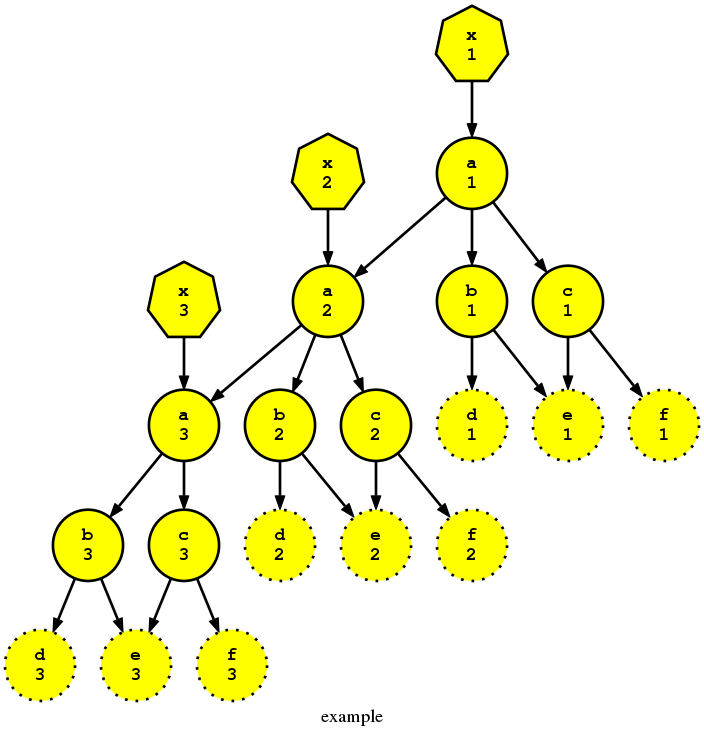
\includegraphics[width=0.45\columnwidth]{resources/example-3cycles.png}
\end{center}

(Note that this can go on indefinitely, and contrast it with separate,
sequential runs of the original single-cycle workflow.)  The task cycle points
(integers here) are just labels, they are not relevant to the scheduling
(except indirectly, insofar as they relate to dependencies). This means cylc
can run workflows faster, recover from delays quicker, and handle failed tasks
better than fixed-cycle schedulers.  The following diagram shows job schedules
for cylc (top) and a traditional fixed-cycle scheduler (bottom) for several
cycles of the example workflow after a delay.

\begin{center}
    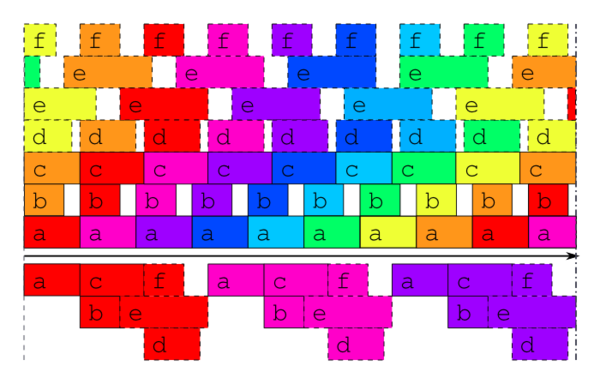
\includegraphics[width=0.55\columnwidth]{resources/tex/timeline-two}
\end{center}
